\documentclass[11pt,a4paper]{article}
\usepackage[a4paper,margin=2.6cm]{geometry}
\usepackage{iftex}
\ifPDFTeX
  \usepackage[T1]{fontenc}
  \usepackage[utf8]{inputenc}
  \usepackage[english]{babel}
\else
  \usepackage{fontspec}
  \usepackage{polyglossia}
  \setdefaultlanguage{english}
  \defaultfontfeatures{Ligatures=TeX}
  \setmainfont{Times New Roman}
  \setsansfont{Arial}
  \setmonofont{Courier New}
\fi
\usepackage{microtype}
\usepackage{mathtools,amssymb}
\usepackage{graphicx}
\usepackage{booktabs}
\usepackage{float}
\usepackage{caption}
\captionsetup{font=small,labelfont=bf}
\usepackage{enumitem}
\setlist{nosep,leftmargin=1.5em}
\usepackage{csquotes}
\usepackage[backend=biber,style=numeric-comp,sorting=none,maxbibnames=6]{biblatex}
\addbibresource{references_v2_en.bib}
\usepackage[unicode,hidelinks]{hyperref}
\setlength{\emergencystretch}{2em}

\title{Regional invariants of the cross-scale organization of the atmospheric circulation:\\
coupling of hierarchical levels and asymmetry of inter-level transfer}
\author{N. Sotiriadi}
\date{2026}

\begin{document}
\maketitle

\begin{abstract}
Hierarchical levels of the organization of geosystems are conventionally identified from the spectral and fractal properties of geographical fields; how the \emph{interaction} between the identified levels should be measured, and whether the pattern of that interaction behaves as an invariant of a territory, has remained an open question. This paper introduces two compact descriptors of the cross-scale organization of the relative vorticity field at the 850~hPa isobaric surface: the level-coupling profile~$P$ (the spatial rank correlation between the activity maps of adjacent octave levels) and the inter-level transfer asymmetry index~$A$ (a measure of the non-reciprocity of the statistical operators of aggregation and refinement). The material is the ERA5 reanalysis for 12 regions of $20^\circ\times40^\circ$ representing six circulation regimes, for the January--March and July--September seasons of 2017--2024; reproducibility is examined against the independent MERRA-2 reanalysis. The study design rests on preregistered criteria, surrogate nulls, and confirmation of every claim on samples that took no part in obtaining it. Both descriptors are shown to form stable regional signatures ($p=0.001$) that persist across seasons, years and ENSO phases. The profile~$P$ is not reducible to the spectral characteristics of levels or to symmetric statistics of cross-scale coupling; the index~$A$ carries information beyond the power spectrum and beyond the profile~$P$, is robust to controls for domain geometry and for the effective resolution of the reanalysis, and its regional geography is reproduced in MERRA-2 with a rank correlation of $\rho=0.93$ ($p<10^{-4}$). The largest values of~$A$ occur over moist-convective oceanic regimes and the smallest over arid continental ones; the Congo and Amazon basins, under a similar regime, exhibit qualitatively different hierarchical architectures. A catalogue of tested and rejected interpretations is given, delimiting the range of valid application of the descriptors. The meaning of inter-level transfer asymmetry as a measurable characteristic of the irreversibility of geographical generalization is discussed.

\smallskip
\noindent\textbf{Keywords:} hierarchical organization of geosystems, invariants, scale, atmospheric circulation, reanalysis, regionalization, generalization.
\end{abstract}

\section{Introduction}
\label{sec:intro}

\subsection{The hierarchy of levels and the problem of invariants}

The view of geosystems as hierarchically organized entities, in which the processes of different spatio-temporal levels are coupled yet not reducible to one another, is among the foundational ideas of Russian theoretical geography. In the work of Yu.\,G.~Puzachenko this idea received an operational development: the spatio-temporal hierarchy of geosystems was examined from the standpoint of oscillation theory \cite{Puzachenko1986}; a mathematical apparatus was assembled for identifying levels of organization from the spectral and fractal properties of geographical fields \cite{Puzachenko2004}; and the search for \emph{invariants of geosystem dynamics} --- temporally stable numerical characteristics of organization that discriminate between territories --- was posed as a research programme in its own right \cite{Puzachenko2010}. An invariant in this sense is not a constant of nature; it is a reproducible measure of how a territory is arranged, one that retains its value as the state of the system changes and is therefore suitable for comparison and regionalization.

This line was carried forward directly by Krenke et al. \cite{Krenke2019}, who identified the hierarchical levels of the organization of a regional mesoclimate from the two-dimensional spectra of the principal components of climatic fields: a power-law (fractal) model of the spectrum served as a background, while departures from it --- breaks in slope and subharmonic peaks --- were interpreted as manifestations of discrete levels with characteristic linear sizes. This answers the question of \emph{where} the levels of organization are located and how strongly each is expressed.

The next question in logical order is how to measure the \emph{interaction} between levels. A hierarchy implies not only the existence of storeys but also definite relations between them: the degree to which the placement of variability at one level is predetermined by the adjacent one, and the directedness of that relation. Quantities of this kind have not so far been constructed as characteristics of a territory in their own right and, accordingly, have not been examined for the status of invariants. The present paper addresses this question for the atmospheric circulation.

\subsection{What existing approaches measure}

Instruments close in spirit have been developed in three international traditions, each of which leaves the quantity we seek outside its scope.

Cascade and multifractal descriptions of atmospheric fields (S.~Lovejoy, D.~Schertzer) have shown that reanalysis fields obey cascade statistics over a wide range of scales and that multifractal exponents are usable as regional climatic characteristics \cite{LovejoySchertzer2013,Lovejoy2011}; the regional and regime dependence of the mesoscale kinetic energy spectrum has likewise been demonstrated by direct computation \cite{Kouhen2024}. Such descriptions characterize the distribution of intensity \emph{along} the scale continuum, but not the spatial consistency of activity maps \emph{between} particular levels.

In the physics of turbulence an apparatus of wavelet decompositions and envelopes has taken shape \cite{Farge1992}. Mathis et al. introduced the amplitude modulation coefficient --- the correlation between a large-scale signal and the envelope of small-scale fluctuations \cite{Mathis2009}; in the statistics of fields the same construction has been systematized as the scattering transform and scattering covariances, that is, statistics of the moduli of wavelet coefficients at pairs of scales \cite{Mallat2012,BrunaMallat2013,Cheng2024}. All these quantities are symmetric by construction: they record the fact of coupling between levels but not its direction. It is telling that the first application of such a technique to geophysical fields for the purpose of discriminating regimes beyond the spectrum appeared only recently and concerns the ocean \cite{Skinner2025}; no climatology of cross-scale level coupling has been constructed for the atmosphere, to our knowledge.

Finally, the literature on atmospheric predictability --- from E.~Lorenz \cite{Lorenz1969} to present-day experiments with global kilometre-scale models \cite{Zhang2007,RotunnoSnyder2008,Judt2020,SelzCraig2023} --- assigns cross-scale interaction the role of a channel through which uncertainty at small scales contaminates the synoptic level and sets regional limits of forecasting. That tradition \emph{models} the strength of cross-scale coupling but does not measure it climatologically from data.

\subsection{Objectives}

(1)~To construct, from the relative vorticity field, two compact descriptors of cross-scale organization: the level-coupling profile~$P$ and the inter-level transfer asymmetry index~$A$. (2)~To examine their status as regional invariants: stability across seasons, years and ENSO phases; irreducibility to the power spectrum, to the spectral characteristics of levels, and to symmetric statistics of cross-scale coupling; and reproducibility in an independent reanalysis. (3)~To delimit the range of valid application, including an account of the interpretations that were tested and rejected. (4)~To discuss the geographical meaning of the resulting quantities in relation to regionalization, generalization, and the assessment of predictability.

\section{Data}
\label{sec:data}

The principal material is the ERA5 reanalysis \cite{Hersbach2020,Soci2024}: the wind components $u$, $v$ at the 850~hPa isobaric surface, on a $0.25^\circ$ grid with a 6~h time step. The choice of the 850~hPa level reflects its representativeness for the lower-tropospheric circulation, which interacts directly with the underlying surface and with convection; the question of the vertical universality of the results is treated separately (Sect.~\ref{sec:limits}).

The analysis is carried out in 12 regions of $20^\circ$ latitude $\times\ 40^\circ$ longitude, selected so as to cover six contrasting circulation regimes (Table~\ref{tab:regions}): tropical oceans (the western Pacific warm pool, the eastern Indian Ocean, the South Pacific Convergence Zone), extratropical storm tracks of both hemispheres (the North Atlantic, the North Pacific, the South Atlantic), centres of deep convection over land (Amazonia, the Congo basin), and continental areas of the temperate and subtropical zones (Europe, Central Asia, Australia, subtropical South America). The time windows are January--March and July--September of three non-overlapping periods: 2017--2019, 2021--2022 and 2023--2024. Each region is represented by eight seasonal windows drawn from two of these periods (the regions introduced at the first stage of the work in 2017--2019 and 2023--2024, the remainder in 2021--2022 and 2023--2024), giving 96 region-windows in total. The periods span opposite ENSO phases (La Ni\~na in 2021--2022, El Ni\~no in 2023--2024), which makes it possible to test the stability of the descriptors not only against changes of season and year but also against a change in the large-scale climatic state.

For an independent test of reproducibility we use the MERRA-2 reanalysis \cite{Gelaro2017}, which is built on a different general circulation model and a different data assimilation system: the wind components at 850~hPa (collection M2I6NPANA, grid $0.5^\circ\times0.625^\circ$, 6~h step) for all 12 regions over 2023--2024 (48 region-windows).

The limitations of the material are stated in advance. The effective resolution of present-day reanalyses amounts to 4--7 grid steps \cite{Skamarock2004,Bolgiani2022}, that is, some 150--200~km for ERA5: variability at smaller scales is shaped to a considerable extent by numerical dissipation and by model parameterizations rather than by resolved dynamics. All the principal conclusions of this work are therefore duplicated by a control restricted to the ``resolved'' levels ($\geq$200~km), and the comparison with MERRA-2, whose grid is twice as coarse, is carried out on those levels only.

\begin{table}[t]
\centering
\caption{Regions of analysis and median values of the inter-level transfer asymmetry index $A$ (decimal logarithm, resolved levels 200--800~km, all windows of 2017--2024).}
\label{tab:regions}
\small
\begin{tabular}{@{}llcc@{}}
\toprule
Region & Bounds & Regime & $A$\\
\midrule
Indian Ocean & $10^\circ$N--$10^\circ$S, $60$--$100^\circ$E & tropical ocean & 2.36\\
Warm pool (WPWP) & $10^\circ$N--$10^\circ$S, $130$--$170^\circ$E & tropical ocean & 2.26\\
South Pacific CZ (SPCZ) & $0$--$20^\circ$S, $180$--$140^\circ$W & tropical ocean & 2.19\\
Australia & $15$--$35^\circ$S, $115$--$155^\circ$E & subtropical continent & 1.80\\
North Pacific & $35$--$55^\circ$N, $180$--$140^\circ$W & storm track & 1.71\\
North Atlantic & $35$--$55^\circ$N, $60$--$20^\circ$W & storm track & 1.67\\
Subtropical S. America & $20$--$40^\circ$S, $75$--$35^\circ$W & subtropical continent & 1.62\\
South Atlantic & $35$--$55^\circ$S, $50$--$10^\circ$W & storm track & 1.59\\
Congo basin & $5^\circ$N--$15^\circ$S, $5$--$45^\circ$E & convective land & 1.58\\
Amazonia & $5^\circ$N--$15^\circ$S, $75$--$35^\circ$W & convective land & 1.53\\
Central Asia & $35$--$55^\circ$N, $60$--$100^\circ$E & arid continent & 1.41\\
Europe & $35$--$55^\circ$N, $10^\circ$W--$30^\circ$E & temperate continent & 1.38\\
\bottomrule
\end{tabular}
\end{table}

\section{Methods}
\label{sec:methods}

\subsection{Octave levels and activity maps}

The working field is the relative vorticity $\omega=\partial v/\partial x-\partial u/\partial y$, computed with allowance for the metric of the sphere (the latitudinal dependence of the longitudinal grid step is treated row by row). Vorticity is preferable to the wind components in that it emphasizes the rotational structure of the flow and suppresses the large-scale advective background.

The decomposition into levels is built by successive Gaussian smoothing with the set of scales $\ell\in\{50,100,200,400,800,1600\}$~km. Level $i$ is defined as the difference between adjacent smoothings,
\begin{equation}
D_i(x,y,t)=\overline{\omega}_{\ell_i}-\overline{\omega}_{\ell_{i+1}},
\end{equation}
and contains structures with characteristic sizes between roughly $\ell_i$ and $\ell_{i+1}$ (an octave), $i=1,\dots,5$. To these is added the residual level $D_0=\omega-\overline{\omega}_{\ell_1}$, which collects everything finer than 50~km. This decomposition corresponds directly to the identification of levels of organization from the spectrum \cite{Krenke2019}, but transfers the analysis from spectral to physical space: for every level an \emph{activity map} (envelope) is constructed,
\begin{equation}
E_i(x,y,t)=\overline{\lvert D_i\rvert}_{\ell_{i+1}},\qquad i=0,\dots,5,
\end{equation}
showing \emph{where} the variability of that level is concentrated at a given time. The use of envelopes as indicators of the local activity of a scale goes back to the wavelet analysis of turbulence \cite{Farge1992}. All spatial statistics are computed over the interior of the domain with a marginal strip excluded, which removes the influence of filtering at the boundaries.

\subsection{Descriptor I: the level-coupling profile}

The level-coupling profile $P=(\rho_1,\dots,\rho_5)$ is defined as the spatial rank (Spearman) correlation between the logarithms of the activity maps of adjacent levels,
\begin{equation}
\rho_i(t)=\operatorname{corr}_{\mathrm{rank}}\!\left[\ln E_{i-1}(\cdot,t),\ \ln E_{i}(\cdot,t)\right],
\label{eq:rho}
\end{equation}
$i=1,\dots,5$, followed by the median over the times of a seasonal window; six activity maps yield five steps of the profile, from the pair (finer than 50; 50--100~km) to the pair (400--800; 800--1600~km). Substantively, $\rho_i$ answers the question of whether the structures of the finer level are active in the same places as those of the adjacent coarser level --- that is, how far the placement of variability at one storey of the hierarchy is predetermined by the adjacent one. The rank form of the correlation makes the descriptor insensitive to any monotone transformation of amplitude, and in particular to regional differences in the overall intensity of the circulation.

One methodological point is essential. The overlap of adjacent Gaussian octaves by itself produces a non-zero coupling even for a random field with the same power spectrum. Alongside the raw profile we therefore consider the \emph{surrogate-referenced excess} $P-P_{\mathrm{surr}}$, where $P_{\mathrm{surr}}$ is the median profile of an ensemble of surrogate fields with the spatial spectrum preserved and the phases randomized. This excess is free of the contribution of filter overlap and reflects the non-Gaussian organization of the field proper.

\subsection{Descriptor II: the inter-level transfer asymmetry index}

The second descriptor addresses the \emph{directedness} of the coupling between levels. For each pair of adjacent octaves, two linear statistical operators are estimated over a sliding time window (20 times, 5~days): the aggregation operator $G^{\uparrow}$, which recovers the state of the coarser level from the finer one, and the refinement operator $G^{\downarrow}$, which recovers the finer level from the coarser one. The operators are built by regression onto the leading spatial modes of the respective octaves with Tikhonov (ridge) regularization.

Were the transition between levels of description statistically reversible, the successive application of these operators would not depend on their order. The measure of departure from reversibility is the norm of their commutator,
\begin{equation}
A_b(t)=\bigl\lVert\,G^{\uparrow}_b G^{\downarrow}_b-G^{\downarrow}_b G^{\uparrow}_b\,\bigr\rVert_F,
\label{eq:A}
\end{equation}
where $b$ is the index of the pair of levels and $\lVert\cdot\rVert_F$ is the Frobenius norm. The resulting characteristic of a region is the median of $\lg A_b$ over times and over the resolved pairs of levels (200--800~km).

Substantively, $A$ measures the \emph{non-reciprocity of aggregation and refinement}. As $A\to0$, the large-scale picture statistically ``remembers'' the arrangement of the mesoscale structure, and the transition between levels of description is close to reversible. Large values of $A$ mean that aggregation irreversibly loses information about the placement of mesoscale variability: it cannot be recovered from the large-scale field even in a statistical sense. We stress the difference from the known characteristics of cross-scale coupling --- the amplitude modulation coefficient \cite{Mathis2009} and scattering covariances \cite{Cheng2024}: the latter are symmetric by construction and by definition do not distinguish the direction in which information is transferred between levels.

\subsection{Design of the statistical testing}

The study follows a falsification-oriented design. The criteria of every stage were fixed \emph{before} the corresponding data were consulted, any departures were logged, and every key claim was confirmed on samples that took no part in obtaining it: for the profile~$P$, on eight regions and on years not used in developing the method; for the index~$A$, on periods untouched by its construction.

The stability of the signatures was assessed by permutation tests of clustering: for the standardized descriptors, median Euclidean distances ``within a region'' (different windows of the same region) and ``between regions'' were compared, with significance determined from 999 permutations of the regional labels. Irreducibility to simpler characteristics was tested by leave-one-out residualization: the part of the descriptor linearly predictable from a control set of features was removed, after which the clustering test was repeated for the residuals. The control sets used in turn were: spectral features (logarithms of the octave variances, the slope of the isotropic spectrum); semi-fractal features --- the slopes and the break position of the power-law model of the spectrum, together with the amplitudes and scales of the peaks of its residuals, that is, direct analogues of the characteristics by which levels are identified in \cite{Krenke2019}; second-order scattering statistics \cite{Cheng2024}; and geometric characteristics of the domains (latitude of the centre, grid step, linear width of the domain), as a possible ``geometric imprint'' of the partitioning scheme.

Surrogate nulls of two kinds were applied in addition: spatial ones (spectrum preserved, phases randomized), to control the contribution of filter overlap, and ones preserving the temporal spectrum of each mode, to control the contribution of temporal autocorrelation in the estimation of the transfer operators. The inertia of the estimator itself was controlled separately: characteristics computed for artificial series with a prescribed autocorrelation and without any cross-level structure set a lower threshold below which observed values were not interpreted.

\section{Results}
\label{sec:results}

\subsection{The level-coupling profile}
\label{sec:results:P}

The profiles $P$ of the twelve regions are shown in Fig.~\ref{fig:profiles}. Three properties constitute the principal result.

\emph{Stability in time.} The curves of the three non-overlapping periods (2017--2019, 2021--2022, 2023--2024), which span opposite ENSO phases, very nearly coincide within each region; the scatter between windows of one region is substantially smaller than the differences between regions.

\emph{Regional discriminability.} A permutation test of clustering confirms the separation of regions on an independent sample ($p=0.001$). Classification of the region from the five-component profile alone yields a proportion of correct assignments of 0.42 against a chance level of $1/12\approx0.08$.

\emph{Shape of the profile.} Coupling decreases systematically from the finer levels to the coarser: adjacent mesoscale levels are tightly coupled ($\rho_1\approx0.84$--$0.91$ virtually everywhere), whereas the coupling with the synoptic level ($\rho_5$) varies widely --- from $0.68$--$0.70$ (the Congo basin, the North and South Atlantic, the warm pool) down to $0.42$--$0.46$ (Amazonia, Europe). It is essential that the ordering of regions by $\rho_5$ does not coincide with their ordering by the asymmetry index (Sect.~\ref{sec:results:A}): the Indian Ocean, for instance, combines the largest value of $A$ with a moderate coupling ($\rho_5=0.52$). This agrees with the formal result on the mutual independence of the two descriptors (Table~\ref{tab:tests}) and means that they describe different aspects of cross-scale organization.

An expansion of the profiles in empirical orthogonal functions shows that 84\,\% of the inter-regional variance falls on a mode concentrated precisely on $\rho_5$; it is natural to call this mode \emph{synoptic decoupling} --- the degree to which the mesoscale organization is detached from synoptic control. The surrogate-referenced excess $P-P_{\mathrm{surr}}$, cleared of the contribution of filter overlap, proves to be non-monotone across levels, with an interior maximum at the second and third steps (scales of 50--400~km): the non-Gaussian consistency of the storeys of the hierarchy proper is greatest in the mesoscale range.

The tests of irreducibility yield a differentiated picture (Table~\ref{tab:tests}). The profile is not explained by the semi-fractal features of the spectrum ($p=0.001$): it measures something beyond the position and the prominence of levels, that is, beyond the information from which levels are identified in \cite{Krenke2019}. Neither is it reducible to scattering statistics ($p=0.026$), the test in the opposite direction being significant as well, so that the two groups of characteristics are mutually complementary; values of $p$ near $0.03$ should nevertheless be regarded as borderline, since windows of one region are not fully independent. With respect to the full power spectrum the conclusion is more guarded: once the geometric characteristics of the domains are included in the control set, the residual clustering loses strict significance ($p=0.10$). In other words, the ``beyond-spectrum'' component of the profile is partly explained by the latitudinal position and the geometry of the domains, and the profile~$P$ should be regarded as a reliable regional signature but only conditionally as a feature independent of the spectrum.

\begin{figure}[t]
\centering

\includegraphics[width=\linewidth]{figures_en/fig_profiles_P.png}
\caption{Level-coupling profiles $P$ for the 12 regions: thin lines are individual seasonal windows, heavy lines the means over the periods 2017--2019, 2021--2022 and 2023--2024. Steps 1--5 correspond to pairs of adjacent levels, from (finer than 50; 50--100~km) to (400--800; 800--1600~km).}
\label{fig:profiles}
\end{figure}

\subsection{The inter-level transfer asymmetry index}
\label{sec:results:A}

The map of the index $A$ (Fig.~\ref{fig:map}) reveals a pronounced and geographically coherent global gradient. The largest values occur in moist-convective oceanic regimes (Indian Ocean 2.36; warm pool 2.26; SPCZ 2.19), intermediate values in the storm tracks (1.59--1.71) and the centres of convection over land (1.53--1.58), and the smallest in arid and temperate continental interiors (Central Asia 1.41; Europe 1.38). The full range spans about one decimal order of magnitude. A ranking of the regions with the interquartile scatter over eight seasonal windows is given in Fig.~\ref{fig:ranking}: the scatter within a region is substantially smaller than the differences between regions, and the ordering of the regions is stable.

The profiles of $A$ across levels (Fig.~\ref{fig:aprofiles}) have a characteristic shape with a maximum in the mesoscale range and are reproduced in all three observation periods; the interannual variations within a region are small compared with the differences between regions.

The statistical standing of the index is the most solid among the results obtained (Table~\ref{tab:tests}). The regional signature is confirmed on a sample of years that took no part in developing the descriptor ($p=0.001$). The index carries information beyond the power spectrum \emph{and} beyond the level-coupling profile $P$ (residualization, $p=0.001$ in both cases): these are different characteristics of organization, not two expressions of one. The result is unchanged when the analysis is restricted to the resolved levels ($\geq$200~km) and when the geometric characteristics of the domains are included in the control set ($p=0.001$ in both cases), so that it is neither an artefact of the sub-grid scales of the reanalysis nor an imprint of the scheme by which the domains were laid out.

An attempt to account for the regional values of $A$ by regression on environmental covariates (mean convective available potential energy, land fraction, orographic variability) yields a formally significant model that is, however, unstable to the exclusion of individual regions. We therefore report the observed regularity --- the asymmetry is greatest for moist convection over the ocean and least over arid land --- as a descriptive characteristic of the geographical distribution rather than as an established functional dependence.

\begin{figure}[t]
\centering

\includegraphics[width=\linewidth]{figures_en/figA_world_map.png}
\caption{The inter-level transfer asymmetry index $A$ (median of the decimal logarithm of the commutator norm over the resolved pairs of levels 200--800~km; ERA5, 850~hPa, all windows of 2017--2024). The numbers are the values of $A$ for the regions.}
\label{fig:map}
\end{figure}

\begin{figure}[t]
\centering

\includegraphics[width=0.93\linewidth]{figures_en/figA_ranking.png}
\caption{Ranking of the regions by the index $A$: bars are medians over the eight seasonal ERA5 windows (2017--2024) with the interquartile scatter; squares are the independent estimate from MERRA-2 (2023--2024).}
\label{fig:ranking}
\end{figure}

\begin{figure}[t]
\centering

\includegraphics[width=\linewidth]{figures_en/figA_profiles.png}
\caption{Profiles of the index $A$ across levels: means over the ERA5 periods (2017--2019, 2021--2022, 2023--2024) and over MERRA-2 (2023--2024, dashed). The grey band marks scales below the effective resolution of the reanalyses; the comparison between reanalyses is carried out on the resolved levels only.}
\label{fig:aprofiles}
\end{figure}

\subsection{Reproducibility in an independent reanalysis}
\label{sec:results:merra}

The decisive test of the nature of the quantities obtained is their reproducibility in a reanalysis built on a different general circulation model and a different assimilation system. Computing both descriptors from MERRA-2 (48 region-windows of 2023--2024, resolved levels) shows that the regional signature of the index $A$ in MERRA-2 is significant ($p=0.001$; likewise $p=0.001$ for the profile $P$), while the regional geography of the index agrees with ERA5 with a rank correlation of $\rho=0.93$ ($p<10^{-4}$; Fig.~\ref{fig:merra}). The ordering of the regions is preserved almost in full, including differences within groups of similar regimes; the systematic offset in level between the reanalyses is attributable to the difference in grids and does not affect the rank agreement.

This rules out an interpretation of the invariant as an artefact of a particular model or of a particular assimilation scheme. What remains common to the two products is the observing network; that limitation is discussed in Sect.~\ref{sec:limits}.

\begin{figure}[t]
\centering

\includegraphics[width=0.62\linewidth]{figures_en/figA_cross_reanalysis.png}
\caption{Reproducibility of the index $A$ in two independent reanalyses: values from ERA5 (abscissa) and MERRA-2 (ordinate) for the 12 regions, 2023--2024, resolved levels 200--800~km.}
\label{fig:merra}
\end{figure}

\subsection{Congo and Amazonia: two regimes of deep convection}
\label{sec:results:congo}

The most telling particular result is the contrast between the two principal centres of deep convection over land. Under a similar overall regime (equatorial land, high convective activity, comparable density of the observing network), the Congo basin exhibits the highest coupling of the mesoscale with the synoptic level among all the regions (median $\rho_5=0.70$), whereas Amazonia exhibits the lowest ($\rho_5=0.42$). The difference is reproduced in all observation periods and is confirmed against MERRA-2; the ranges of values over individual windows ($0.57$--$0.81$ and $0.36$--$0.54$ respectively) do not overlap over the greater part of their extent.

Qualitatively the same picture is visible in the activity maps of the levels (Fig.~\ref{fig:octaves}). In the storm track the frontal structure can be traced consistently across all storeys of the hierarchy, from the mesoscale octaves to the synoptic ones: knowing the large-scale field, one can say where the small-scale activity is concentrated. In the Amazonian regime the maps of the coarse levels barely predict the placement of mesoscale variability: the convective organization is formed predominantly ``from below''.

Two centres of convection that are close in climatic regime and in integral characteristics thus correspond to \emph{different architectures} of cross-scale organization --- a difference detected neither by spectra nor by standard convective indices, yet recorded consistently by the proposed descriptors. The physical mechanism of the contrast (the relative roles of easterly waves, vertical wind shear, the diurnal cycle of convection, and the orographic framing of the basins) constitutes a separate problem of regional analysis.

\begin{figure}[t]
\centering
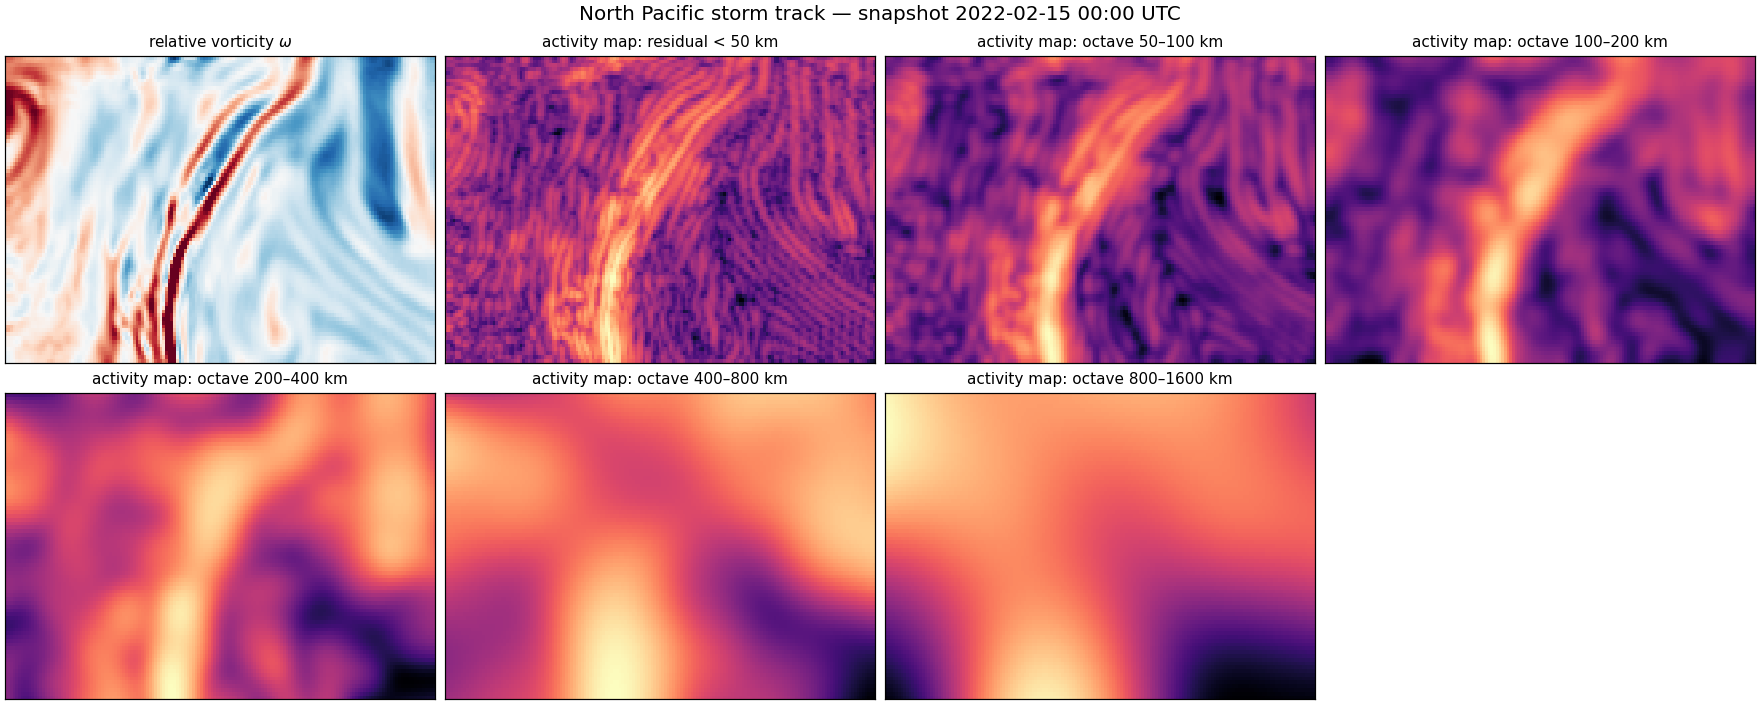
\includegraphics[width=\linewidth]{figures_en/octave_maps_R9_NPAC.png}\\[3pt]
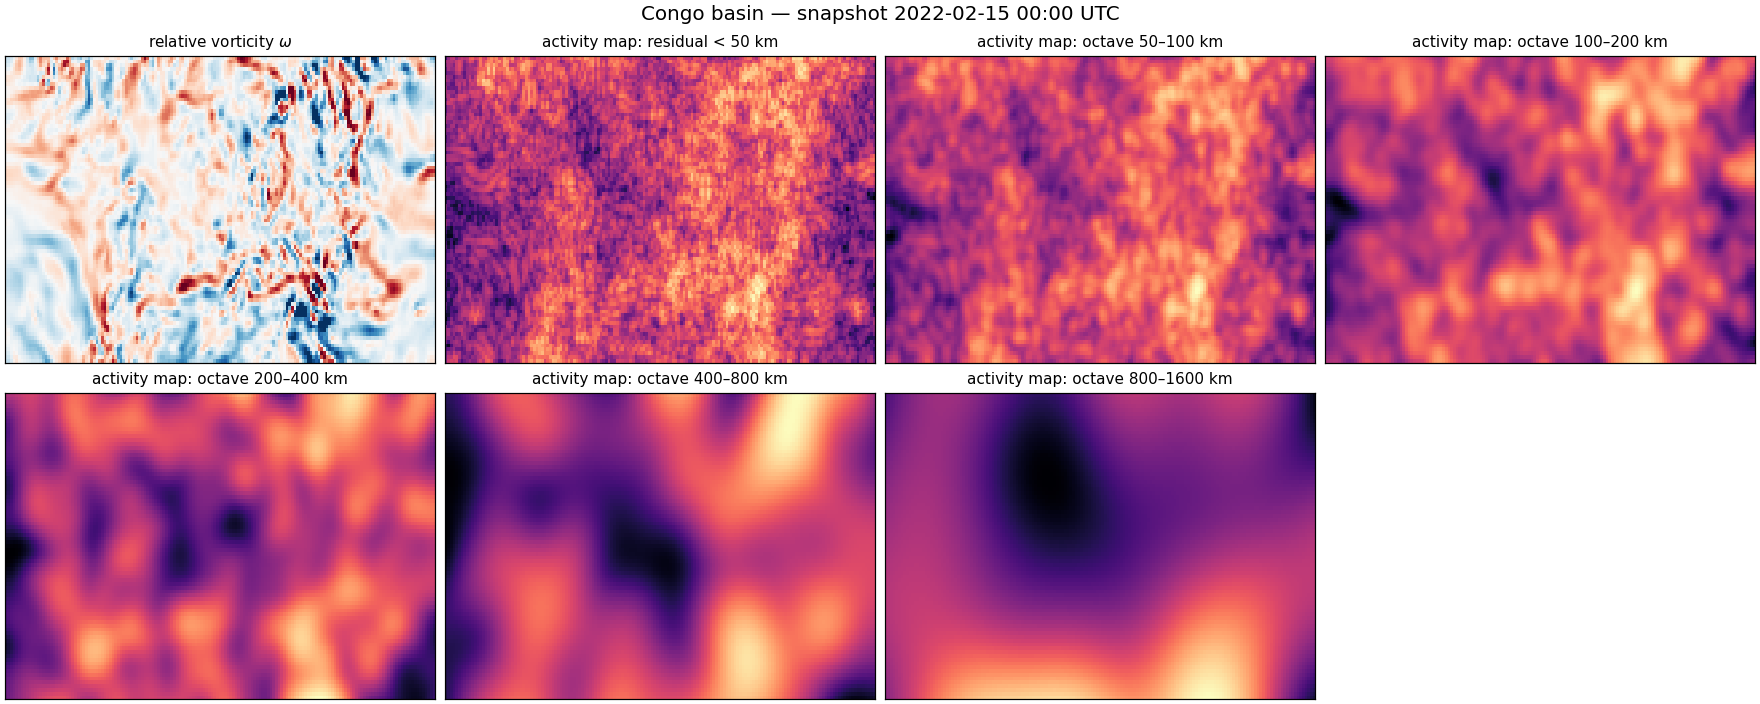
\includegraphics[width=\linewidth]{figures_en/octave_maps_R7_CONGO.png}
\caption{Activity maps of the octave levels at a single time (15 February 2022): above, the North Pacific (the frontal structure appears consistently at all levels, high coupling); below, the Congo basin (mesoscale activity is less subordinated to the coarse levels). The colour scale of each panel is individual (logarithm of the envelope): the coupling measures the coincidence of the geography of activity, not of its amplitude.}
\label{fig:octaves}
\end{figure}

\begin{table}[t]
\centering
\caption{Summary of the tests of the descriptors. Significance levels of permutation tests of clustering are given (999 permutations of the regional labels); ``independent years'' denotes samples that took no part in constructing the descriptor concerned.}
\label{tab:tests}
\small
\begin{tabular}{@{}p{0.40\linewidth}p{0.27\linewidth}p{0.25\linewidth}@{}}
\toprule
Test & Profile $P$ & Index $A$\\
\midrule
Regional signature, independent years & $p=0.001$ & $p=0.001$\\
Beyond the power spectrum & $p=0.029$; with geometry control $p=0.10$ & $p=0.001$; with geometry control $p=0.001$\\
Beyond the semi-fractal characteristics of levels \cite{Krenke2019} & $p=0.001$ & ---\\
Beyond scattering statistics \cite{Cheng2024} & $p=0.026$ & ---\\
Beyond the profile $P$ & --- & $p=0.001$\\
Coarse levels only (steps $\rho_3$--$\rho_5$; bands from 200~km) & $p=0.002$ & $p=0.001$\\
Signature in MERRA-2 & $p=0.001$ & $p=0.001$\\
Agreement of ERA5 / MERRA-2 geography & --- & $\rho=0.93$; $p<10^{-4}$\\
\bottomrule
\end{tabular}
\end{table}

\section{Range of valid application}
\label{sec:limits}

Alongside the confirmed properties of the descriptors, a number of possible interpretations were tested and rejected. We report them in full (Table~\ref{tab:negative}), since they delimit the domain in which the proposed quantities may correctly be used and forestall their over-interpretation.

\emph{The descriptors should not be understood as a measure of the cross-scale flux of kinetic energy.} A scalar contraction of the same transfer operators, compared directly against the flux computed by spatial coarse-graining \cite{Germano1992,Aluie2018} (the implementation was verified on a numerical experiment with a known solution), accounts for fractions of a per cent of its variability ($R^2=0.003$--$0.007$) as against $0.35$--$0.47$ for standard characteristics of the resolved strain field. The asymmetry of cross-scale information transfer and the transfer of energy across the spectrum are distinct properties of the flow, and the proposed descriptors characterize the former, not the latter.

\emph{No simple law relating the shape of the profiles to environmental covariates was found.} Neither a renormalization of the scale axis by a characteristic size determined from the spectral break, nor removal of zonal banding, nor a change to the field of vertically integrated water vapour transport brings the profiles of different regions onto a single curve; the last of these transformations in fact accentuates the inter-regional differences. Nor was a predictor of the synoptic decoupling mode found among latitude, vertical wind shear, convective potential, land fraction and orographic variability.

\emph{There is no instantaneous local relation between the index $A$ and precipitation.} When the domains are subdivided into cells and the series within them compared, no relation is present. At the regime level (five-day smoothing) a stable negative correlation between $A$ and precipitation appears, together with a lagged structure with a characteristic time of about two days, consistent with the known cycle of consumption and recovery of convective available energy \cite{Masunaga2012,PetersNeelin2006}. An attempt to formalize this as a dynamical ``source--sink'' equation did not, however, survive testing on independent regions, and the characteristic time is partly reproduced by the inertia of the estimator itself; we therefore confine ourselves to noting the agreement of time scales and do not assert a causal relation.

\emph{No vertical universality was found.} At the 500~hPa level the regional signature of the index is not statistically confirmed ($p=0.18$), and the agreement with the geography of the 850~hPa level is not significant ($\rho=0.43$, $p=0.17$); this sample is half the size of the principal one, so the correct formulation is an absence of confirmation rather than a demonstrated difference. In any case the quantities obtained should be referred to a particular isobaric surface; the construction of a vertically integrated descriptor is a separate task.

\emph{The descriptors carry no information about the residual of the moisture budget.} The residual of the moisture budget equation in a reanalysis is governed chiefly by assimilation increments \cite{Trenberth1991,Mayer2021}, and adding cross-scale characteristics of the circulation to the standard set of predictors does not improve its description.

\emph{The consistency of the transfer operators does not exceed the level set by temporal autocorrelation.} Testing against surrogates that preserve the temporal spectrum of each mode showed that the observed consistency of the successive application of the aggregation and refinement operators along different paths in the ``time--scale'' space is accounted for by the autocorrelation of the fields; there are no grounds for speaking of any consistent geometric structure of transfer. The index $A$ is to be understood precisely as an empirical measure of non-reciprocity, and not as an element of a geometric construction.

\begin{table}[t]
\centering
\caption{Interpretations of the descriptors that were tested and rejected.}
\label{tab:negative}
\small
\begin{tabular}{@{}p{0.55\linewidth}p{0.39\linewidth}@{}}
\toprule
Proposition tested & Outcome\\
\midrule
The descriptors track the cross-scale flux of kinetic energy & rejected (standard characteristics of the strain field are two orders of magnitude more informative)\\
The shape of the profiles obeys a universal law in environmental covariates & rejected (no collapse onto a single curve under any of three renormalizations)\\
A predictor of the synoptic decoupling mode exists among environmental characteristics & not found\\
The index $A$ is instantaneously and locally related to precipitation & rejected (no relation at the level of cells)\\
The regime-level relation of $A$ to precipitation is formalizable as a ``source--sink'' equation & not established (no predictive power on independent regions)\\
The descriptors are vertically universal (transfer to 500~hPa) & rejected (level specificity)\\
The descriptors are informative for closing the moisture budget of a reanalysis & rejected (median gain in quality $-0.018$; $p=0.92$)\\
The transfer operators form a consistent structure beyond temporal autocorrelation & rejected (test against surrogates with the temporal spectrum preserved)\\
\bottomrule
\end{tabular}
\end{table}

\section{Discussion}
\label{sec:discussion}

\subsection{The geographical meaning of the quantities obtained}

The proposed descriptors characterize what may naturally be called the \emph{architecture of the hierarchy} of a regional circulation regime. The profile $P$ answers the question of how far the placement of mesoscale variability is subordinated to the coarse levels; the index $A$, of how irreversible the transition between levels of description is.

The latter admits a direct interpretation in terms of the classical geographical problem of generalization. Generalization --- the passage to a coarser level of description of a territory --- is always accompanied by a loss of information; the question is \emph{how that loss is organized}. Small values of $A$ mean that the lost detail remains statistically ``addressed'': from the large-scale picture one can say where the mesoscale variability is concentrated, and statistical refinement has a basis. Large values of $A$ mean the opposite: the mesoscale organization is generated by processes weakly determined by the large-scale field, and generalization is irreversible in the strong sense. The observed geographical distribution --- a maximum over moist-convective oceans and a minimum over arid continents --- accords with the intuitive view of moist convection as a source of mesoscale organization that is not reducible to synoptic control.

Two applied areas follow. The first is objective regionalization by the type of cross-scale organization: the descriptors provide a compact, reproducible feature of a regime that discriminates even between territories with similar spectral characteristics, as the contrast between the Congo and Amazon basins shows. The second is an a~priori assessment of how well founded statistical refinement (downscaling) is: regions with large values of $A$ are those in which the recovery of mesoscale structure from large-scale fields is least warranted, irrespective of the refinement method employed.

In terms of the programme of searching for invariants \cite{Puzachenko2010}, the characteristics obtained satisfy the operational definition: they are stable in time (seasons, years, ENSO phases), they discriminate between territories, they are reproduced in independent data sources, and they are not reducible to previously known characteristics of organization --- spectra, fractal dimensions, and the spectral features of levels \cite{Krenke2019}. We regard the present work as a continuation of that same line: from the identification of hierarchical levels to the measurement of their interaction.

\subsection{A hypothesis on the relation to predictability}

The literature on forecast error growth assigns cross-scale interaction the role of a channel through which uncertainty at small scales contaminates the synoptic level and limits predictability \cite{Lorenz1969,Zhang2007,RotunnoSnyder2008,Judt2020}. The regional climatology of that interaction constructed here gives rise to a testable hypothesis: regional differences in the coupling and in the asymmetry of levels should correspond to regional differences in the rate of error growth in ensemble forecasting systems, with regimes of high asymmetry and weak synoptic coupling exhibiting a faster loss of predictability. We state this as a hypothesis: testing it requires ensemble data and constitutes a separate task.

\subsection{Limitations}

The principal limitation in principle is the dependence, common to all reanalyses, on the observing network. Reproducibility of the invariant in two independent assimilation systems rules out an artefact of a particular model, but not an artefact of the geography of observations as such: both systems assimilate largely the same data, and the density of observations differs between ocean and land, and between the tropics and the temperate latitudes \cite{BonavitaLaloyaux2020,Soci2024}. Removing this limitation entirely would require computing the descriptors from free-running (non-assimilating) model experiments at high resolution.

The remaining limitations are listed above: the analysis was performed for a single isobaric surface (level specificity is shown directly), for two seasons and for a fixed layout of domains; scales finer than $\sim$200~km lie below the effective resolution of the reanalyses and are excluded from the conclusions; and finally, the descriptors remain statistical characteristics --- a dynamical model generating the observed regional differences has not been constructed.

\section{Conclusions}
\label{sec:conclusion}

1.~Two compact descriptors of the cross-scale organization of the atmospheric circulation are proposed: the level-coupling profile $P$, which characterizes the degree to which mesoscale variability is subordinated to the coarse levels, and the inter-level transfer asymmetry index $A$, which characterizes the irreversibility of the transition between levels of description. The latter, unlike the known characteristics of cross-scale coupling, distinguishes the direction in which information is transferred between levels.

2.~Both descriptors form stable regional signatures that persist across seasons, years and ENSO phases ($p=0.001$ on samples that took no part in their construction). The profile $P$ is not reducible to the spectral characteristics of levels ($p=0.001$) or to symmetric statistics of cross-scale coupling, while its independence of the full power spectrum is conditional. The index $A$ carries information beyond the power spectrum and beyond the profile $P$ ($p=0.001$) and is robust to controls for domain geometry and for the effective resolution of the reanalysis.

3.~The regional geography of the index $A$ is reproduced in the independent MERRA-2 reanalysis with a rank correlation of $\rho=0.93$: the property measured pertains to the atmosphere and not to the data assimilation system. The maximum of the asymmetry occurs in moist-convective oceanic regimes and the minimum in arid continental ones; the Congo and Amazon basins, under a similar regime, exhibit qualitatively different architectures of the hierarchy.

4.~The range of valid application is delimited: the descriptors do not measure the flux of kinetic energy, do not obey a simple law in environmental covariates, are level-specific, and carry no information about the residual of a reanalysis moisture budget; the regime-level agreement with the cycle of convective energy is not formalizable as a dynamical equation.

5.~The characteristics obtained satisfy the operational definition of an invariant of geosystem dynamics and continue the line of research into hierarchical organization --- from the identification of levels to the measurement of their interaction. The nearest applications are objective regionalization by the type of cross-scale organization and an a~priori assessment of how well founded statistical refinement is; a testable hypothesis relating the quantities obtained to regional limits of predictability has been formulated.

\paragraph{Data and code.} The testing protocols, the program code, the full table of the experiments performed and the numerical results are openly available at \url{https://github.com/Theclimateguy/Shroedinger}.

\printbibliography[title={References}]

\end{document}
